We describe a realistic setting where we can obtain small, in average, HL for the CSP.
We need few overpasses, which are edges connecting long shortest paths in a costly zone.
Let us denote the costly edges as $\Ec\defeq\crl{e\in E:c_e>0}$.

\begin{definition}[Overpass]
For $r>0$, an edge $e=(u,v)$ is an $r$-overpass if: (1) both $u$ and $v$ are endpoints of paths in $\PS_{r(2-\St)/\St}$, (2) $\min(\dist(e,\Ec),\dist(\Ec,e))\leq 3r/2$ and (3) $e$ belongs to a path $Q\in\PE_{2r}\setminus\PS$.
\end{definition} 

If costs are contiguous, i.e.\ they lay on a shortest path, such as the case of tolls in highways or traffic jumps, then the notion of overpass corresponds to the intuitive concept, see \cref{fig:overpass} for an explanation.
For every scale $r>0$, we ask for a \emph{bounded growth} condition controlling the number of $r$-overpasses.
We also assume that edges are shortest paths between its endpoints, this property is clearly obeyed by road networks.

\begin{definition}(Bounded Growth)
$(G,c,\ell)$ satisfies the bounded growth condition if, $\forall r>0$, $\abs{\crl{u\in V: \exists v, uv \text{ is an $r$-overpass}}}\leq \phi(2r)$, where $\phi(r)\defeq nh\alpha^{\beta-2-\log_2r}$
\end{definition}

Observe that $\phi$ is a slowly decreasing function of $r$ and, even when $r=D$, we allow for overpasses.
With these conditions we can prove the following.

\begin{figure}
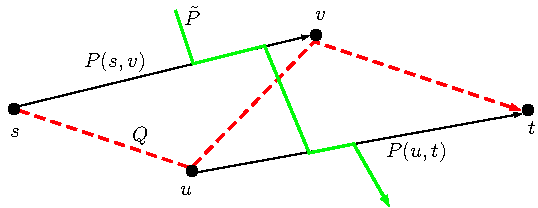
\includegraphics[scale=0.6]{TexImg/overpass.pdf}
\caption{There is a contiguous path $\tilde P$ (solid green) with cost. 
The efficient path $Q$ (dashed red) uses edge $uv$, but avoids both the shortest paths $P(s,v)$ and $P(u,t)$.
Edge $uv$ is an overpass, because their endpoints meet long shortest paths around a costly zone.} 
\label{fig:overpass}
\end{figure}

\begin{theorem}\label{theo:overpasses}
Let $(G,\ell,c)$ be a network with HD $h$.
If the bounded growth is satisfied, we can obtain, in polynomial time, HL for the CSP to answer queries in average time $\Or((b+1)\alpha h'\log D)$ and with total storage $\Or(nB\cdot B\alpha h'\log D)$, where $h'=\Or(\Delta h\log(hn\Delta))$.
\end{theorem}

We refer to the average HD of $\PE$ as average CHD.
We discussed that average HD is enough to obtain good preprocessing algorithms, therefore an average CHD should intuitively suffice.
To prove \cref{theo:overpasses} we  need to show that it is possible to obtain small average CHD under even less restrictive assumptions than the partial-witness.
We will allow for an additional \emph{lay witness set} $D$ such that, whenever a path $P$ does not have a good subpath, we can exhibit $v\in D$ hitting $P$.
This correspond to the intuition that a few bad efficient paths should not completely ruin the algorithm. 

\begin{definition}[Weak Partial Witness]
Let $\beta\geq 0$.
We say that a path system  $\calQ$ is weakly $\beta$-witnessed by the path system $\calQ'$ if, for every $r>0$, $\exists D_r\subseteq V$ such that, $\forall Q\in \calQ_r$ either (1) $Q$ is $\beta$-witnessed by $\calQ'$ or (2) $Q$ is hit by $D_r$.
Additionally we require $\abs{D_r}\leq \phi(r)$.
\end{definition} 

Intuitively, the lay witness set $D_r$ takes care of all the corner cases where $\calQ$ and $\calQ'$ differ too much.
We now show that our requirement on $\abs{D_r}$ guarantees a bound on the average HD.

\begin{proposition}\label[proposition]{prop:lay_witness}
Assume that $G$ is $\alpha$-doubling and let $\calQ'$ be weakly $\beta$-witnessed by $\calQ$.
If the HD of $\calQ$ is $h$, then the average HD of $\calQ'$ is $h'\leq 2\alpha^{\beta}h$
\end{proposition}
\begin{proof}
Let $r>0$, and $C$ be an $(h,2^{-\beta}r)$-LSHS for $\calQ$.
We show that $C\cup D_r$ is an average $(h,r)$-LSHS for $\calQ'$.
Clearly is a hitting set for $\calQ'_r$ and we can compute
\begin{align*}
h'&\leq \frac{1}{n}\sum_{v\in V} \abs{B_{2r}(v)\cap (C\cup D_r)}\\
&\leq \frac{1}{n}\prn*{\sum_{v\in V} \abs{B_{2r}(v)\cap C}+\sum_{v\in V} \abs{B_{2r}(v)\cap D_r}}\\
&\leq \frac{1}{n}\prn*{\sum_{v\in V} \alpha^\beta h+\sum_{v\in D_r} \abs{B_{2r}(v)}}
\leq \alpha^\beta h + \frac{\abs{D_r}\alpha^{\log_2r+2}}{n}.
\end{align*}
In the third inequality we used that $C$ is sparse with respect to balls of radius $2^{-\beta+1}r$ and that $\sum_{v\in V} \abs{B_{2r}(v)\cap D_r}=\sum_{v\in D_r} \abs{B_{2r}(v)}$ by symmetry of the bi-directional balls.
In the last inequality we used that, by doubling dimension, balls of radius $r$ have at most $\alpha^{\log_2r+1}$ elements.
Since $\abs{D_r}\leq \phi(r)$, the result follows.
\end{proof}

To prove the next result, we will need the following notation.
For a path $Q$ and two vertices $u,v\in Q$ we denote $Q[u,v]\subseteq Q$ as the sub $(u,v)$-path.
For two paths $P,Q$, we denote $P|Q$ as the concatenation, which is defined only when $P,Q$ share the correct endpoint.

\begin{proposition}\label[proposition]{prop:1witness}
With bounded growth, $\PS$ is a weak $1$-witness for $\PE$.
\end{proposition}
\begin{proof}
Let $Q\in\PE$, call its endpoints $s,t$ and set $\ell(Q)=2r$.
We will show how to obtain a vertex for the lay witness set in case $Q$ is not witnessed and then we bound the size of the set.
Assume that $Q\neq P(s,t)$, otherwise the path is trivially witnessed.
Let $(u,v)\in Q$ be such that $\ell(Q[s,v]),\ell(Q[u,t])\geq r$. 
If either $Q[s,v]$ or $Q[u,t]$ is a shortest path or $\ell_{uv}\geq r$, then $Q$ is witnessed, so we assume that all of these fail.
See \cref{fig:overpass} for a diagram.

We claim that $uv$ is a $r$-overpass.
Condition 1 of an overpass is satisfied because either $Q[s,v]$ or $Q[u,t]$ have stretch at most $\frac{2-\St}{\St}$.
To see this, note that both $P(s,v)|Q[v,t]$ and $Q[s,u]|P(u,t)$ are no shorter than $P(s,t)$ and $\St\ell(P(s,t))\geq \ell(Q)$, hence
$\frac{2r}{\St}\leq \ell(P(s,t)) \leq  \ell(P(s,v)) + \ell(Q[v,t])$ and $\frac{2r}{\St} \leq \ell(P(s,t)) \leq  \ell(Q[s,u]) + \ell(P(u,t))$.
Since each path $Q[s,u],Q[v,t]$ has length less than $r$, it follows that both $P(s,v),P(u,t)$ have length strictly greater than $\frac{2-\St}{\St}r$ and condition 1 follows. 
Finally, to show condition 2, we have $\ell(Q[s,v])+\ell(Q[u,t])=r+\ell_{uv}$ and since $\ell_{uv}<r/2$, one of $Q[s,v]$ or $Q[u,t]$ has length at most $3r/4$.
Since neither of these paths is shortest, it most be that both $P(s,v),P(u,t)$ have costly edges and thus one of $u,v$ is closer than $3r/4$ to $E_1$ and the condition is satisfied.

For every path of length $2r$, we can either exhibit a witness or show that it contains an overpass and add use the tail of the edge as a lay witness.
For a fixed $r>0$, we need to add as many $\phi(r)$ nodes to $D_r$ to cover all the efficient paths. 
The result follows.
\end{proof}

We are almost ready to prove that bounded growth allows to solve the CSP.
The last piece is \cref{theo:avg_chd}, whose proof is far from trivial, but we already gave the construction with the augmented graph.
The arguments mimic those in \cref{theo:HLeff,theo:preproc_avg}.

\begin{theorem}\label{theo:avg_chd}
If the average HD of $\PE$ is $h_c$, then we can obtain, in polynomial time, HL to answer queries with budget $b$ in average time $\Or((b+1)h_c'\log D)$ and the space requirements are $\Or(nB\cdot Bh_c'\log D)$.
\end{theorem}

\begin{proofof}{\cref{theo:overpasses}}
We argue that the average CHD is $h_c\leq 2\alpha h$.
By \cref{prop:1witness}, $\PE$ is weakly $1$-witnessed by $\PS$.
It follows by \cref{prop:lay_witness} that the average CHD is at most $2\alpha h$ as needed.
Applying \cref{theo:avg_chd} yields the result.
\end{proofof}